Questa sezione riguarda la definizione della topologia di rete in Mininet e la conseguente suddivisione in due \textit{slices} isolati. Lo scopo è costruire una topologia secondo la quale gli host possono comunicare attraverso rotte predefinite:
\begin{itemize}
    \item L'host h1 può comunicare solo con h3 tramite il path superiore;
    \item L'host h2 può comunicare solo con h4 tramite il path inferiore.
\end{itemize}

\noindent
A questo proposito, è stata definita la seguente configurazione Mininet implementando il costruttore della classe Mininet.Environment, la cui vista logica è rappresentata in figura \ref{img:network_view}.

\vspace{.5cm}
\begin{pythoncode}[]
class Environment(object):
    def __init__(self):
    # ... 
    # Definizione hosts
    self.h1 = self.net.addHost('h1', mac= '00:00:00:00:00:01', ip= '10.0.0.1')
    self.h2 = self.net.addHost('h2', mac= '00:00:00:00:00:02', ip= '10.0.0.2')
    self.h3 = self.net.addHost('h3', mac= '00:00:00:00:00:03', ip= '10.0.0.3')
    self.h4 = self.net.addHost('h4', mac= '00:00:00:00:00:04', ip= '10.0.0.4')

    # Definizione switch
    self.s1 = self.net.addSwitch('s1')
    self.s2 = self.net.addSwitch('s2')
    self.Up = self.net.addSwitch('s3') # up
    self.Dw = self.net.addSwitch('s4') # down

    # Link declaration 
    self.net.addLink(self.h1, self.s1, delay='0.01ms', port1=1, port2=1)
    self.net.addLink(self.h2, self.s1, delay='0.01ms', port1=1, port2=2)
    self.net.addLink(self.h3, self.s2, delay='0.01ms', port1=1, port2=3)
    self.net.addLink(self.h4, self.s2, delay='0.01ms', port1=1, port2=4)
    self.net.addLink(self.s1, self.Up, bw=10, delay='0.025ms', port1=3, port2=1)
    self.net.addLink(self.Up, self.s2, bw=10, delay='0.025ms', port1=2, port2=1)
    self.net.addLink(self.s1, self.Dw, bw=1, delay='0.025ms', port1=4, port2=1)
    self.net.addLink(self.Dw, self.s2, bw=1, delay='0.025ms', port1=2, port2=2)
    # ...
\end{pythoncode}

\begin{figure}[ht]
    \centering
    \setlength{\fboxrule}{.5pt} 
    \setlength{\fboxsep}{3pt} 
    \fbox{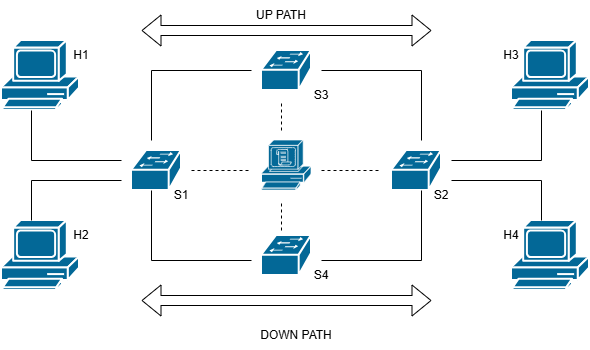
\includegraphics[width=0.8\textwidth]{img/network_view.png}}
    \label{img:network_view}
\end{figure}

\begin{pythoncode}
# Estensione della classe base
class RyuController(app_manager.RyuApp):
    # OpenFlow 1.3 (Rifiuta linguaggi precedenti)
    OFP_VERSIONS = [ofproto_v1_3.OFP_VERSION]

    def __init__(self, *args, **kwargs):
        super(RyuController, self).__init__(*args, **kwargs)
        
        self.h1 = '00:00:00:00:00:01'
        self.h2 = '00:00:00:00:00:02'
        self.h3 = '00:00:00:00:00:03'
        self.h4 = '00:00:00:00:00:04'

    # Installa una flow rule OpenFlow nello switch
    def add_flow(self, datapath, priority, match, actions, idle_timeout=0, flag=0):
        ofproto = datapath.ofproto
        parser = datapath.ofproto_parser

        inst = [parser.OFPInstructionActions(ofproto.OFPIT_APPLY_ACTIONS, actions)]
        mod = parser.OFPFlowMod(
            datapath=datapath, priority=priority,
            match=match, instructions=inst,
            idle_timeout = idle_timeout, flags=flag
        )

        # invio della regola allo switch
        datapath.send_msg(mod)
\end{pythoncode}

\noindent
Date le ridotte dimensioni della rete, sono state inserite delle regole nel controllore che impongono le rotte. 
\begin{info}
    RyuController è un controller SDN OpenFlow 1.3 basato su Ryu che usa Mininet e Open vSwitch. \uppercase{è} stato implementato a partire dalla classe base ryu.base.app\_manager.RyuApp, e gli indirizzi MAC degli host sono stati inseriti come stringhe statiche direttamente nel costruttore.
\end{info}

\noindent
Quando Mininet avvia uno switch, questo prova ad aprire una connessione TCP verso il controller Ryu. Se la connessione viene stabilita (handshake a tre vie), viene avviato l'handshake OpenFlow. Dopodichè, lo switch invia un messaggio FEATURES\_REPLY, ed il controller esegue switch\_features\_handler.

\newpage
\begin{pythoncode}
@set_ev_cls(ofp_event.EventOFPSwitchFeatures, CONFIG_DISPATCHER)
def switch_features_handler(self, ev):
    datapath = ev.msg.datapath
    ofproto = datapath.ofproto
    parser = datapath.ofproto_parser
    dpid = datapath.id

    if dpid == 1:
        # UP flow 
        port_out_Up = 3
        port_in_Up = 1

        # Flow IN
        self.add_mac_flow(datapath, self.h1, self.h3, port_out_Up)
        self.add_arp_flow(datapath, self.h1, port_out_Up)

        # Flow Back
        self.add_mac_flow(datapath, self.h3, self.h1, port_in_Up)
        self.add_arp_flow(datapath, self.h3, port_in_Up)

        # Down flow configuration 
        port_out_Dw = 4
        port_in_Dw = 2
        
        # Flow IN
        self.add_mac_flow(datapath, self.h2, self.h4, port_out_Dw)
        self.add_arp_flow(datapath, self.h2, port_out_Dw)

        # Flow Back
        self.add_mac_flow(datapath, self.h4, self.h2, port_in_Dw)
        self.add_arp_flow(datapath, self.h4, port_in_Dw)

    elif dpid == 2:
        port_out_Up = 1
        port_in_Up = 3

        self.add_mac_flow(datapath, self.h3, self.h1, port_out_Up)
        self.add_arp_flow(datapath, self.h3, port_out_Up)

        self.add_mac_flow(datapath, self.h1, self.h3, port_in_Up)
        self.add_arp_flow(datapath, self.h1, port_in_Up)

        port_out_Dw = 2
        port_in_Dw = 4
        
        self.add_mac_flow(datapath, self.h4, self.h2, port_out_Dw)
        self.add_arp_flow(datapath, self.h4, port_out_Dw)

        self.add_mac_flow(datapath, self.h2, self.h4, port_in_Dw)
        self.add_arp_flow(datapath, self.h2, port_in_Dw)

    elif dpid == 3:
        port_1 = 1
        port_2 = 2

        self.add_mac_flow(datapath, self.h1, self.h3, port_2)
        self.add_arp_flow(datapath, self.h1, port_2)

        self.add_mac_flow(datapath, self.h3, self.h1, port_1)
        self.add_arp_flow(datapath, self.h3, port_1)
    
    elif dpid == 4:
        port_1 = 1
        port_2 = 2

        self.add_mac_flow(datapath, self.h2, self.h4, port_2)
        self.add_arp_flow(datapath, self.h2, port_2)

        self.add_mac_flow(datapath, self.h4, self.h2, port_1)
        self.add_arp_flow(datapath, self.h4, port_1)    
        
\end{pythoncode}

\noindent
Dopo aver determinato l'identità dello switch con \textit{dpid}, il controller crea la regola attraverso add\_mac\_flow, ovvero l'associazione (mac\_src, mac\_dst) $\rightarrow$ port. Attraverso la regola add\_arp\_flow, imponiamo che i messaggi ARP possono uscire su più porte, ed è una regola a priorità più alta di quella che impone il flusso basato su MAC. Osserviamo che comunque il pacchetto ARP, che viene inviato in broadcast, viene comunque confinato nello \textit{slice} della rete. 

\vspace{.3cm}
\begin{pythoncode}
    def add_mac_flow(self, datapath, src, dst, out_port, priority=10):
        parser = datapath.ofproto_parser

        match = parser.OFPMatch(eth_src=src, eth_dst=dst)
        actions = [parser.OFPActionOutput(out_port)]
        self.add_flow(datapath, priority, match, actions)
    
    def add_arp_flow(self, datapath, eth_src, out_port):
        parser = datapath.ofproto_parser
        
        match = parser.OFPMatch(eth_src=eth_src, eth_dst="ff:ff:ff:ff:ff:ff", eth_type=0x0806)
        actions = []
        if not isinstance(out_port, list):
            out_port = [out_port]

        for port in out_port:
            actions.append(parser.OFPActionOutput(port))
        self.add_flow(datapath, priority=20, match=match, actions=actions)

\end{pythoncode}

\noindent
Per testare questa configurazione sono stati usati i tool \textit{pingall} di Mininet e \textit{Whireshark}.

\begin{commandline}
\begin{verbatim}
mininet> pingall 
*** Ping: testing ping reachability

h1 -> X h3 X 
h2 -> X X h4 
h3 -> h1 X X 
h4 -> X h2 X

*** Results: 66% dropped (4/12 received) 
\end{verbatim}
\end{commandline}

\begin{figure}[ht]
    \centering
    \setlength{\fboxrule}{.5pt} 
    \setlength{\fboxsep}{3pt} 
    \fbox{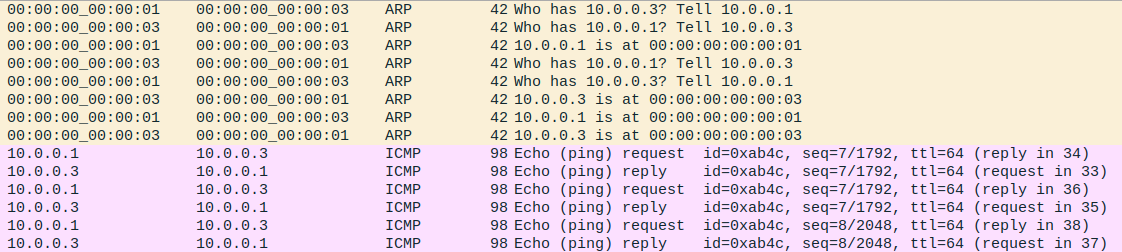
\includegraphics[width=0.9\textwidth]{img/T_whireshark_h1toh3.png}}
    \label{img:h1toh3}
\end{figure}

\begin{figure}[ht]
    \centering
    \setlength{\fboxrule}{.5pt} 
    \setlength{\fboxsep}{3pt} 
    \fbox{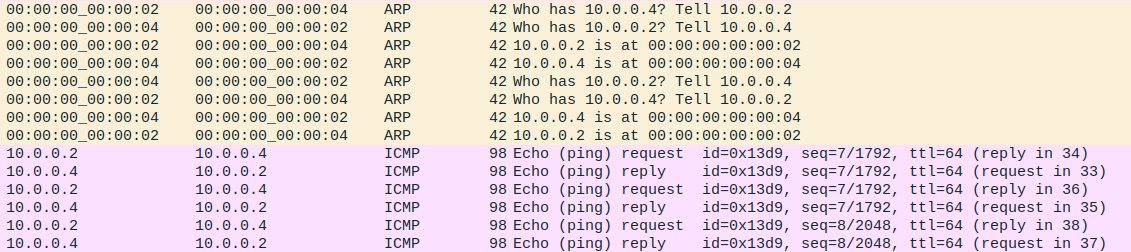
\includegraphics[width=0.9\textwidth]{img/T_whireshark_h2toh4.png}}
    \label{img:h2toh4}
\end{figure}
